%%%%%%%%%%%%%%%%%%%%%%%%%%%%%%%%%%%%%%%%%%%%%%%%%%%%%%%%%%%%%%%%%%%%%%%%%%%%%%%%
%2345678901234567890123456789012345678901234567890123456789012345678901234567890
%        1         2         3         4         5         6         7         8

\documentclass[letterpaper, 10 pt, conference]{ieeeconf}  % Comment this line out if you need a4paper

%\documentclass[a4paper, 10pt, conference]{ieeeconf}      % Use this line for a4 paper

\IEEEoverridecommandlockouts                              % This command is only needed if 
                                                          % you want to use the \thanks command

\overrideIEEEmargins                                      % Needed to meet printer requirements.

%In case you encounter the following error:
%Error 1010 The PDF file may be corrupt (unable to open PDF file) OR
%Error 1000 An error occurred while parsing a contents stream. Unable to analyze the PDF file.
%This is a known problem with pdfLaTeX conversion filter. The file cannot be opened with acrobat reader
%Please use one of the alternatives below to circumvent this error by uncommenting one or the other
%\pdfobjcompresslevel=0
%\pdfminorversion=4

% See the \addtolength command later in the file to balance the column lengths
% on the last page of the document

% The following packages can be found on http:\\www.ctan.org
%\usepackage{graphics} % for pdf, bitmapped graphics files
%\usepackage{epsfig} % for postscript graphics files
%\usepackage{mathptmx} % assumes new font selection scheme installed
%\usepackage{times} % assumes new font selection scheme installed
\usepackage{amsmath} % assumes amsmath package installed
\usepackage{amssymb}  % assumes amsmath package installed

\usepackage{url}
\usepackage{multirow}
\usepackage{makecell}
\usepackage{booktabs}
\usepackage{changepage}
\usepackage{balance}
\usepackage[dvipsnames]{xcolor}
\usepackage[dvipdfmx]{graphicx}

\newcommand{\figref}[1]{{Fig.~\ref{#1}}}
\newcommand{\tabref}[1]{{Table~\ref{#1}}}
\newcommand{\bm}[1]{\mbox{\boldmath{$#1$}}}
\newcommand{\TODO}[1]{\fbox{{\bf TODO}#1}}
%% \usepackage{pifont}
%% \newcommand{\yesmark}{\textcolor{ForestGreen}{\ding{51}}}
%% \newcommand{\nomark}{\textcolor{BrickRed}{\ding{55}}}
\newcommand{\yesmark}{\textcolor{ForestGreen}{Yes}}
\newcommand{\nomark}{\textcolor{BrickRed}{No}}
\newcommand{\partialmark}{\textcolor{Orange}{Partial}}
\renewcommand{\thefootnote}{\fnsymbol{footnote}}

\title{\LARGE \bf
  RoboManipBaselines: A Unified Framework for Imitation Learning in Robotic Manipulation across Real and Simulated Environments
}

\author{
Masaki Murooka$^{1,2}$, Tomohiro Motoda$^{1}$, Ryoichi Nakajo$^{1}$, \\Hanbit Oh$^{1}$, Koshi Makihara$^{1}$, Keisuke Shirai$^{1}$, Yukiyasu Domae$^{1}$% <-this % stops a space
\thanks{$^{1}$Artificial Intelligence Research Center,
National Institute of Advanced Industrial Science and Technology (AIST),
2-3-26 Aomi, Koto-ku, Tokyo 135-0064, Japan.
{\tt\small m-murooka@aist.go.jp}}%
\thanks{$^{2}$CNRS-AIST JRL (Joint Robotics Laboratory), IRL,
1-1-1 Umezono, Tsukuba, Ibaraki 305-8560, Japan.}%
}

\begin{document}

\maketitle
\thispagestyle{empty}
\pagestyle{empty}

%% floatsep is 12.0pt plus 2.39996pt minus 2.39996pt (= 12.0pt)
%% textfloatsep is 20.39996pt plus 2.39996pt minus 4.79993pt (= 18.0pt)
%% abovecaptionskip is 6.0pt
%% abovedisplayskip is 6.74997pt plus 4.0pt minus 2.0pt (= 8.74997pt)
%% belowdisplayskip is 6.74997pt plus 4.0pt minus 2.0pt (= 8.74997pt)
\setlength{\floatsep}{8pt}
\setlength{\textfloatsep}{8pt}
\setlength{\abovecaptionskip}{4pt}
\setlength{\abovedisplayskip}{4pt}
\setlength{\belowdisplayskip}{4pt}

%%%%%%%%%%%%%%%%%%%%%%%%%%%%%%%%%%%%%%%%%%%%%%%%%%%%%%%%%%%%%%%%%%%%%%%%%%%%%%%%
\begin{abstract}
\end{abstract}

\begin{keywords}
  Deep Learning in Grasping and Manipulation; Imitation Learning; Software Tools for Benchmarking and Reproducibility
\end{keywords}

%%%%%%%%%%%%%%%%%%%%%%%%%%%%%%%%%%%%%%%%%%%%%%%%%%%%%%%%%%%%%%%%%%%%%%%%%%%%%%%%
\section{Introduction}

In recent years, learning-based approaches that generate robot motions directly from demonstration data have attracted increasing attention.
Such approaches rely on data collection as well as model training and execution, and therefore require software functionalities that differ fundamentally from those of conventional model-based approaches.
At the same time, efforts to apply learning-based motion generation to industrial and service domains are expanding, particularly for tasks that have been difficult to automate using conventional methods.
However, compared to programming or direct teaching, learning-based approaches involve unique pipelines for deployment, making verification and practical adoption more challenging.

In this paper, we introduce \textbf{RoboManipBaselines}, a general-purpose open framework for robot learning developed to address these challenges\footnote{\url{https://github.com/isri-aist/RoboManipBaselines}}.
As illustrated in \figref{fig:overview}, RoboManipBaselines is designed to advance both research and real-world deployment of robot imitation learning, with emphasis on the following four principles:
\begin{itemize}
\item \textbf{Integration}: providing an end-to-end workflow from data collection to policy training and rollout
\item \textbf{Generality}: supporting diverse environments in both simulation and the real world
\item \textbf{Extensibility}: allowing new robots, tasks, and policy models to be added with minimal effort
\item \textbf{Reproducibility}: enabling systematic benchmarking with publicly available datasets
\end{itemize}
These features support fair benchmarking and efficient experimentation across multiple methods.

A comparison with other open frameworks~\cite{Robomimic:Mandlekar:CoRL2021,LIBERO:Liu:NeurIPS2023,Maniskill:Tao:RSS2025,RoboHive:Kumar:NeurIPS2023,RoboCasa:Nasiriany:RSS2024,D3IL:Jia:ICLR2024,Colosseum:Pumacay:RSS2024,LeRobot:Cadene:GitHub2024,RoboVerse:Geng:RSS2025} is summarized in \tabref{tab:comparison}.
RoboManipBaselines offers a wide range of capabilities for robot imitation learning.

\begin{figure}[tb]
  \centering
  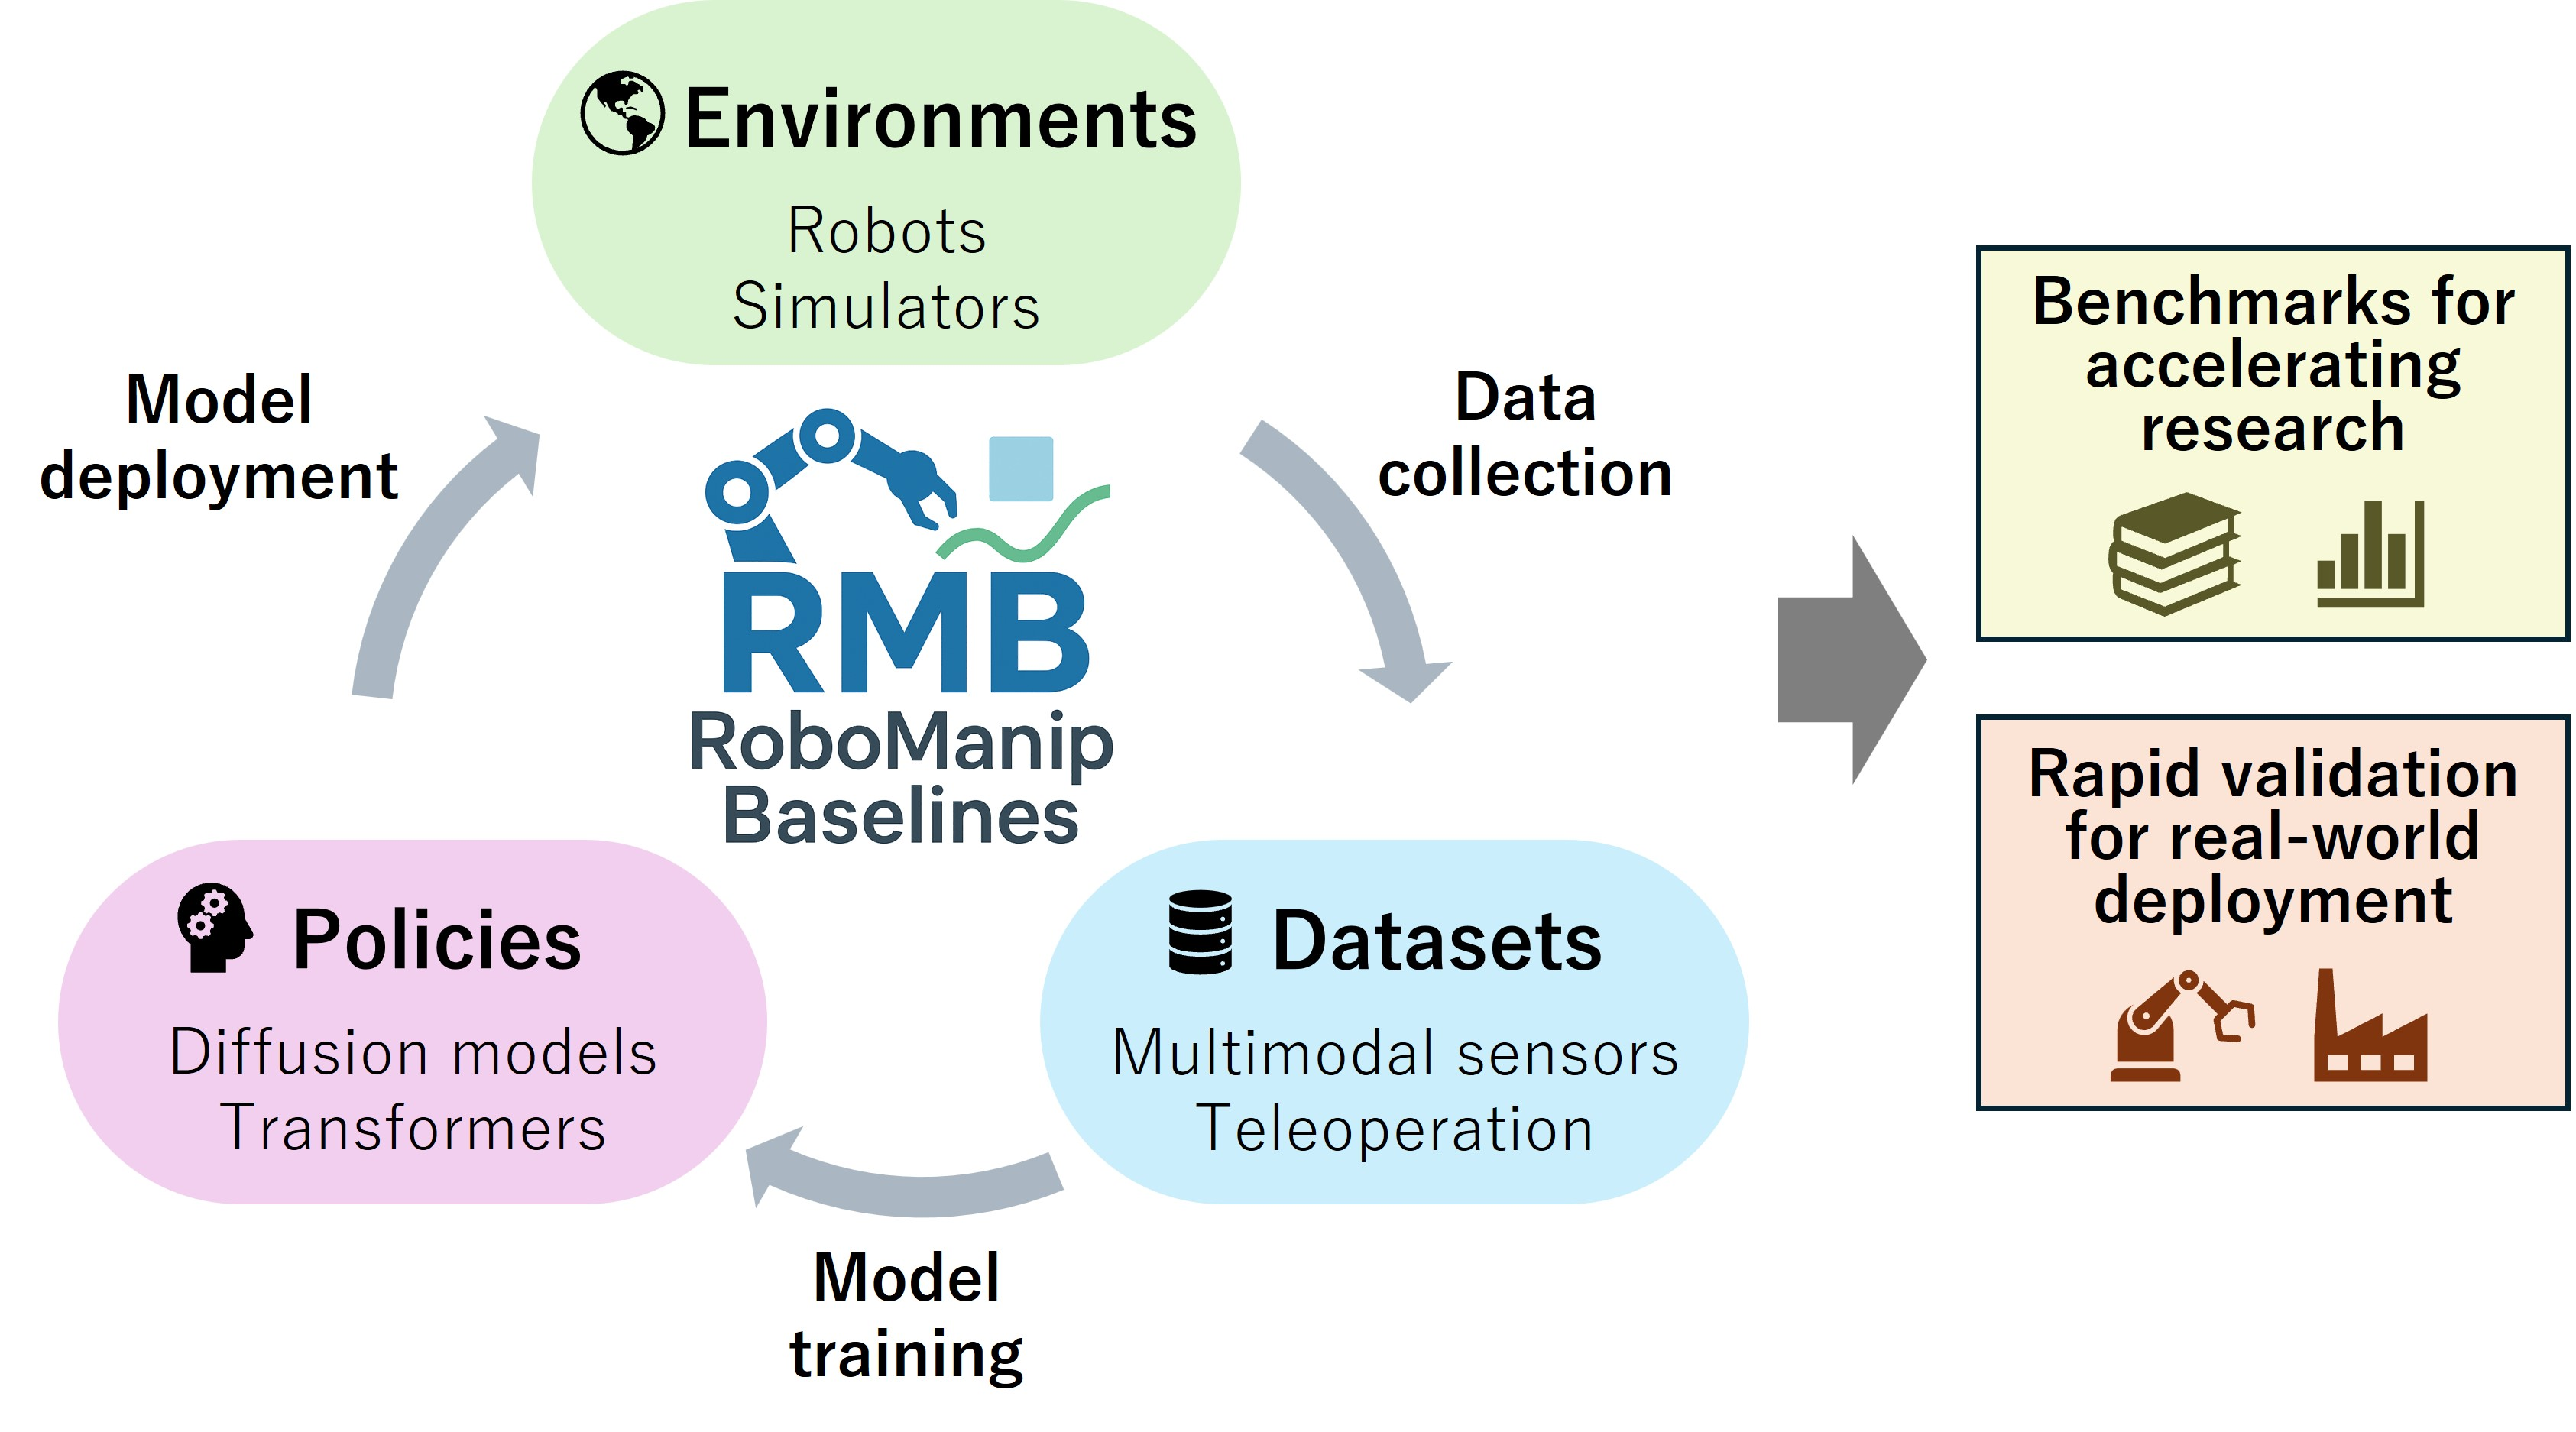
\includegraphics[width=0.99\columnwidth]{figs/overview2.jpg}
  \caption{Overview of RoboManipBaselines.}
  \label{fig:overview}
\end{figure}

\begin{table*}[tb]
  \centering
  \renewcommand{\arraystretch}{1.2}
  \caption{Comparison of open frameworks for robot learning.}
  \label{tab:comparison}
  \resizebox{\textwidth}{!}{
    \begin{tabular}{lccccccccc}
      \toprule
      \multirow{2}{*}{\textbf{Framework}} & \multicolumn{3}{c}{\textbf{Environments}} & \multicolumn{2}{c}{\textbf{Embodiments}} & \multicolumn{2}{c}{\textbf{Multimodal Sensors}} & \multicolumn{2}{c}{\textbf{Policy Models}} \\
      \cmidrule(lr){2-4} \cmidrule(lr){5-6} \cmidrule(lr){7-8} \cmidrule(lr){9-10}
      & Real-world & Simulators & \makecell{Deformable\\ objects} & Bimanual & Mobile & Tactile & Point clouds & \makecell{3D} & \makecell{Language-\\conditioned} \\
      \midrule
      robomimic~\cite{Robomimic:Mandlekar:CoRL2021} & \partialmark$^1$ & MuJoCo & \nomark & \yesmark & \partialmark$^2$ & \nomark & \nomark & \nomark & \yesmark \\
      LIBERO~\cite{LIBERO:Liu:NeurIPS2023} & \nomark & MuJoCo & \nomark & \nomark & \nomark & \nomark & \nomark & \nomark & \yesmark \\
      ManiSkill~\cite{Maniskill:Tao:RSS2025} & \nomark & SAPIEN & \nomark & \yesmark & \yesmark & \nomark & \yesmark & \nomark & \nomark \\
      RoboHive~\cite{RoboHive:Kumar:NeurIPS2023} & \yesmark & MuJoCo & \yesmark & \yesmark & \yesmark & \nomark & \yesmark & \nomark & \nomark \\
      RoboCasa~\cite{RoboCasa:Nasiriany:RSS2024} & \partialmark$^1$ & MuJoCo & \nomark & \yesmark & \yesmark & \nomark & \yesmark & \nomark & \yesmark \\
      D3IL~\cite{D3IL:Jia:ICLR2024} & \nomark & MuJoCo & \nomark & \nomark & \nomark & \nomark & \nomark & \nomark & \nomark \\
      COLOSSEUM~\cite{Colosseum:Pumacay:RSS2024} & \yesmark & CoppeliaSim & \yesmark & \nomark & \nomark & \nomark & \yesmark & \yesmark & \yesmark \\
      LeRobot~\cite{LeRobot:Cadene:GitHub2024} & \yesmark & MuJoCo & \nomark & \yesmark & \yesmark & \nomark & \nomark & \nomark & \yesmark \\
      RoboVerse~\cite{RoboVerse:Geng:RSS2025} & \yesmark & 7 simulators & \yesmark & \yesmark & \yesmark & \yesmark & \yesmark & \nomark & \yesmark \\
      \textbf{RoboManipBaselines} & \yesmark & MuJoCo, Isaac Gym & \yesmark & \yesmark & \yesmark & \yesmark & \yesmark & \yesmark & \yesmark \\
      \bottomrule
    \end{tabular}
  }
  \\
  \vspace{3mm}
  \begin{adjustwidth}{10pt}{0pt}
    \raggedright
    %% \yesmark \ indicates supported, \nomark \ indicates not supported, \partialmark \ indicates limited support.\\
    $^1$ While the framework has been applied to real robots in some reports, it does not fully support the end-to-end workflow from data collection to model deployment across multiple robot types.\\
    $^2$ An external dataset for mobile manipulators, MOMART~\cite{MOMART:Wong:CoRL2022}, has been released in a format compatible with robomimic. However, mobile manipulators are not directly supported within robomimic itself.
  \end{adjustwidth}
\end{table*}


%%%%%%%%%%%%%%%%%%%%%%%%%%%%%%%%%%%%%%%%%%%%%%%%%%%%%%%%%%%%%%%%%%%%%%%%%%%%%%%%
\section{Problem Formulation}

We first describe the problem formulation of robot imitation learning considered in RoboManipBaselines.
The environment $\mathcal{E}$ is defined by the state space $\mathcal{S}$, the action space $\mathcal{A}$, and the state transition function $f : \mathcal{S} \times \mathcal{A} \to \mathcal{S}$.
At time step $t$, the robot observes a state $s_t \in \mathcal{S}$ and selects an action $a_t \in \mathcal{A}$, which leads to the next state $s_{t+1} = f(s_t, a_t)$.

In imitation learning, multiple trajectories of state-action pairs $\tau = \{(s_t, a_t)\}_{t=1}^{T}$ are first collected, from which a dataset $\mathcal{D} = \{\tau^{(i)}\}_{i=1}^{N}$ is constructed.
Based on this dataset, a policy $\pi : \mathcal{S} \to \mathcal{A}$ is trained to map states to actions.
The policy $\pi$ is typically represented by a neural network and trained using supervised learning.

%%%%%%%%%%%%%%%%%%%%%%%%%%%%%%%%%%%%%%%%%%%%%%%%%%%%%%%%%%%%%%%%%%%%%%%%%%%%%%%%
\section{Framework Design}

\begin{figure*}[tb]
  \centering
  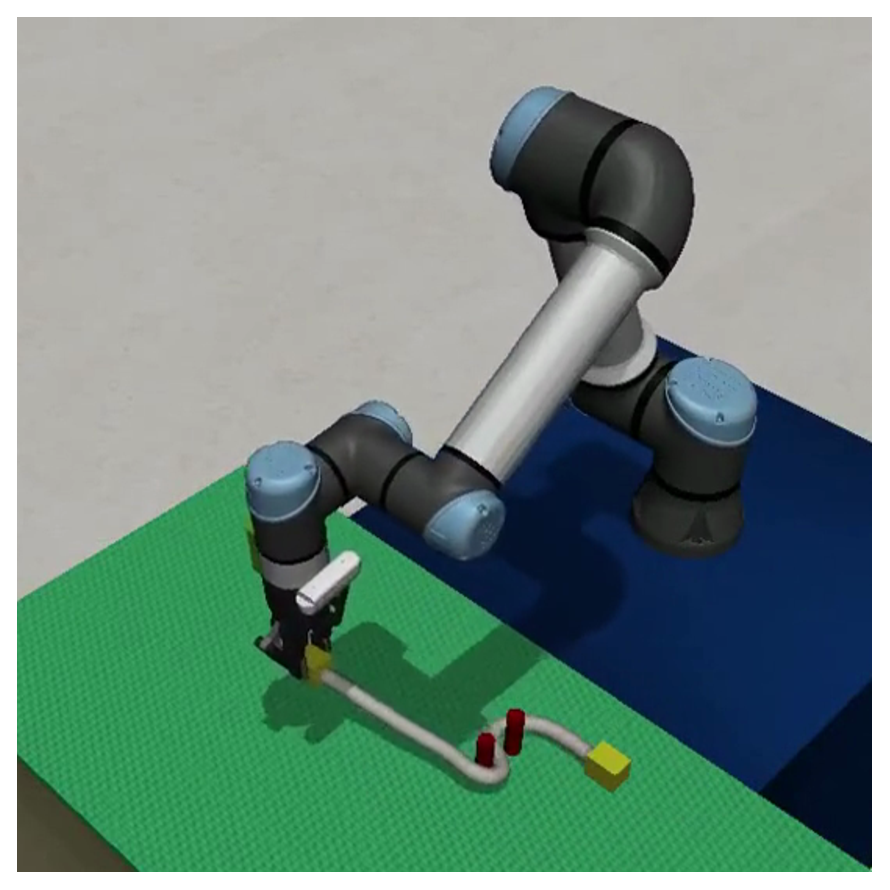
\includegraphics[width=0.16\textwidth]{figs/mujoco_ur5e.eps}
  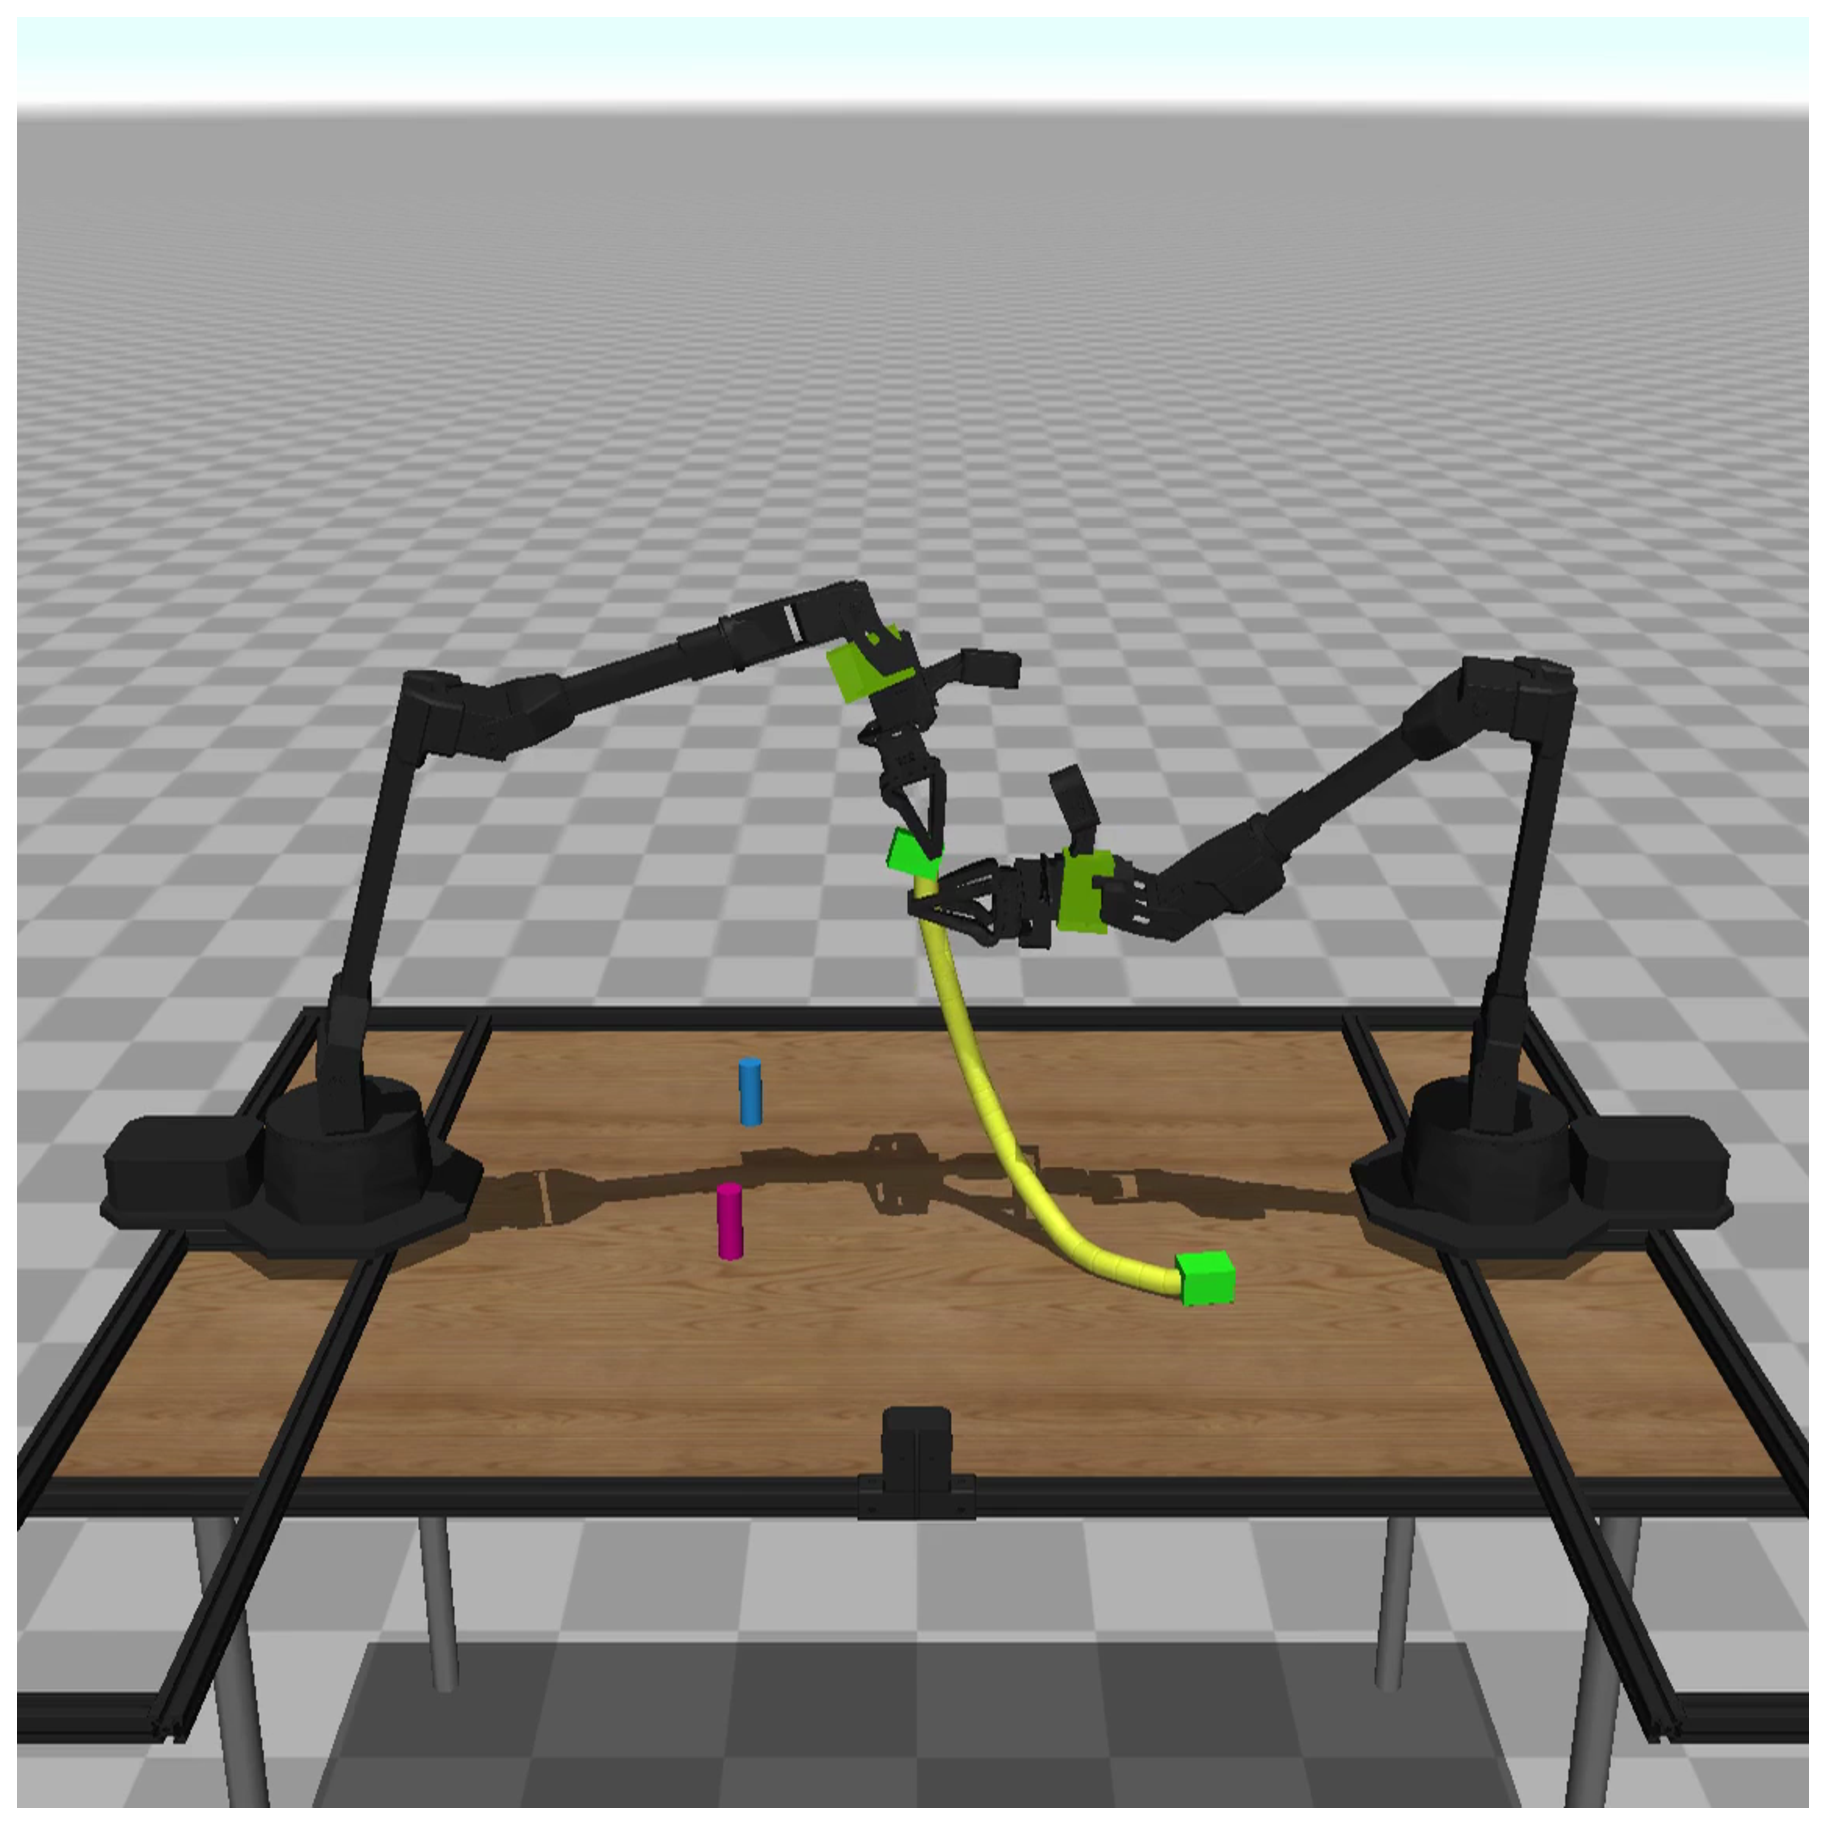
\includegraphics[width=0.16\textwidth]{figs/mujoco_aloha.eps}
  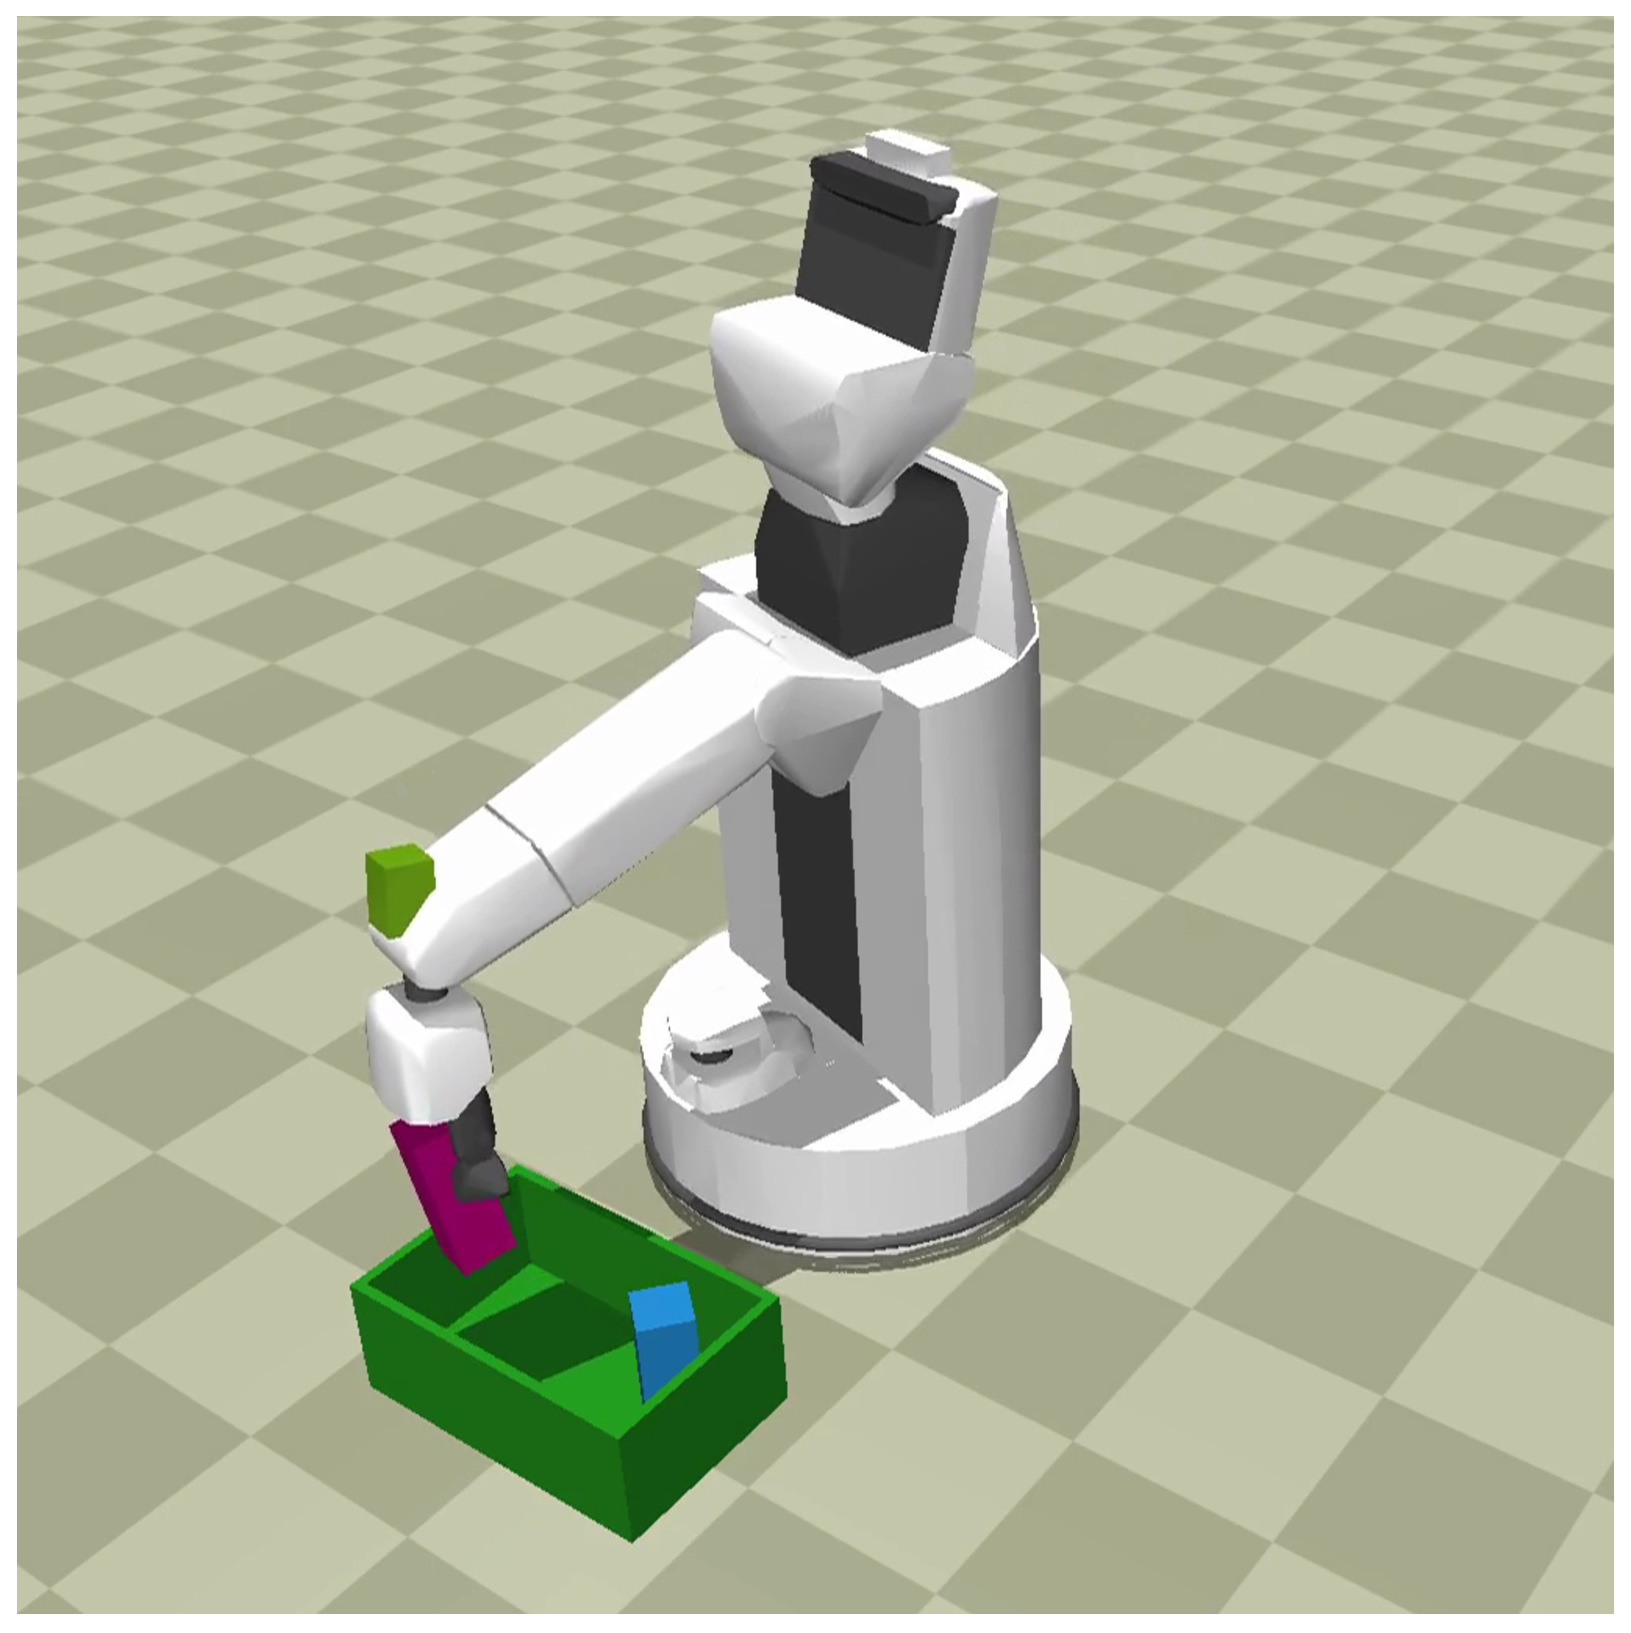
\includegraphics[width=0.16\textwidth]{figs/mujoco_hsr.eps}
  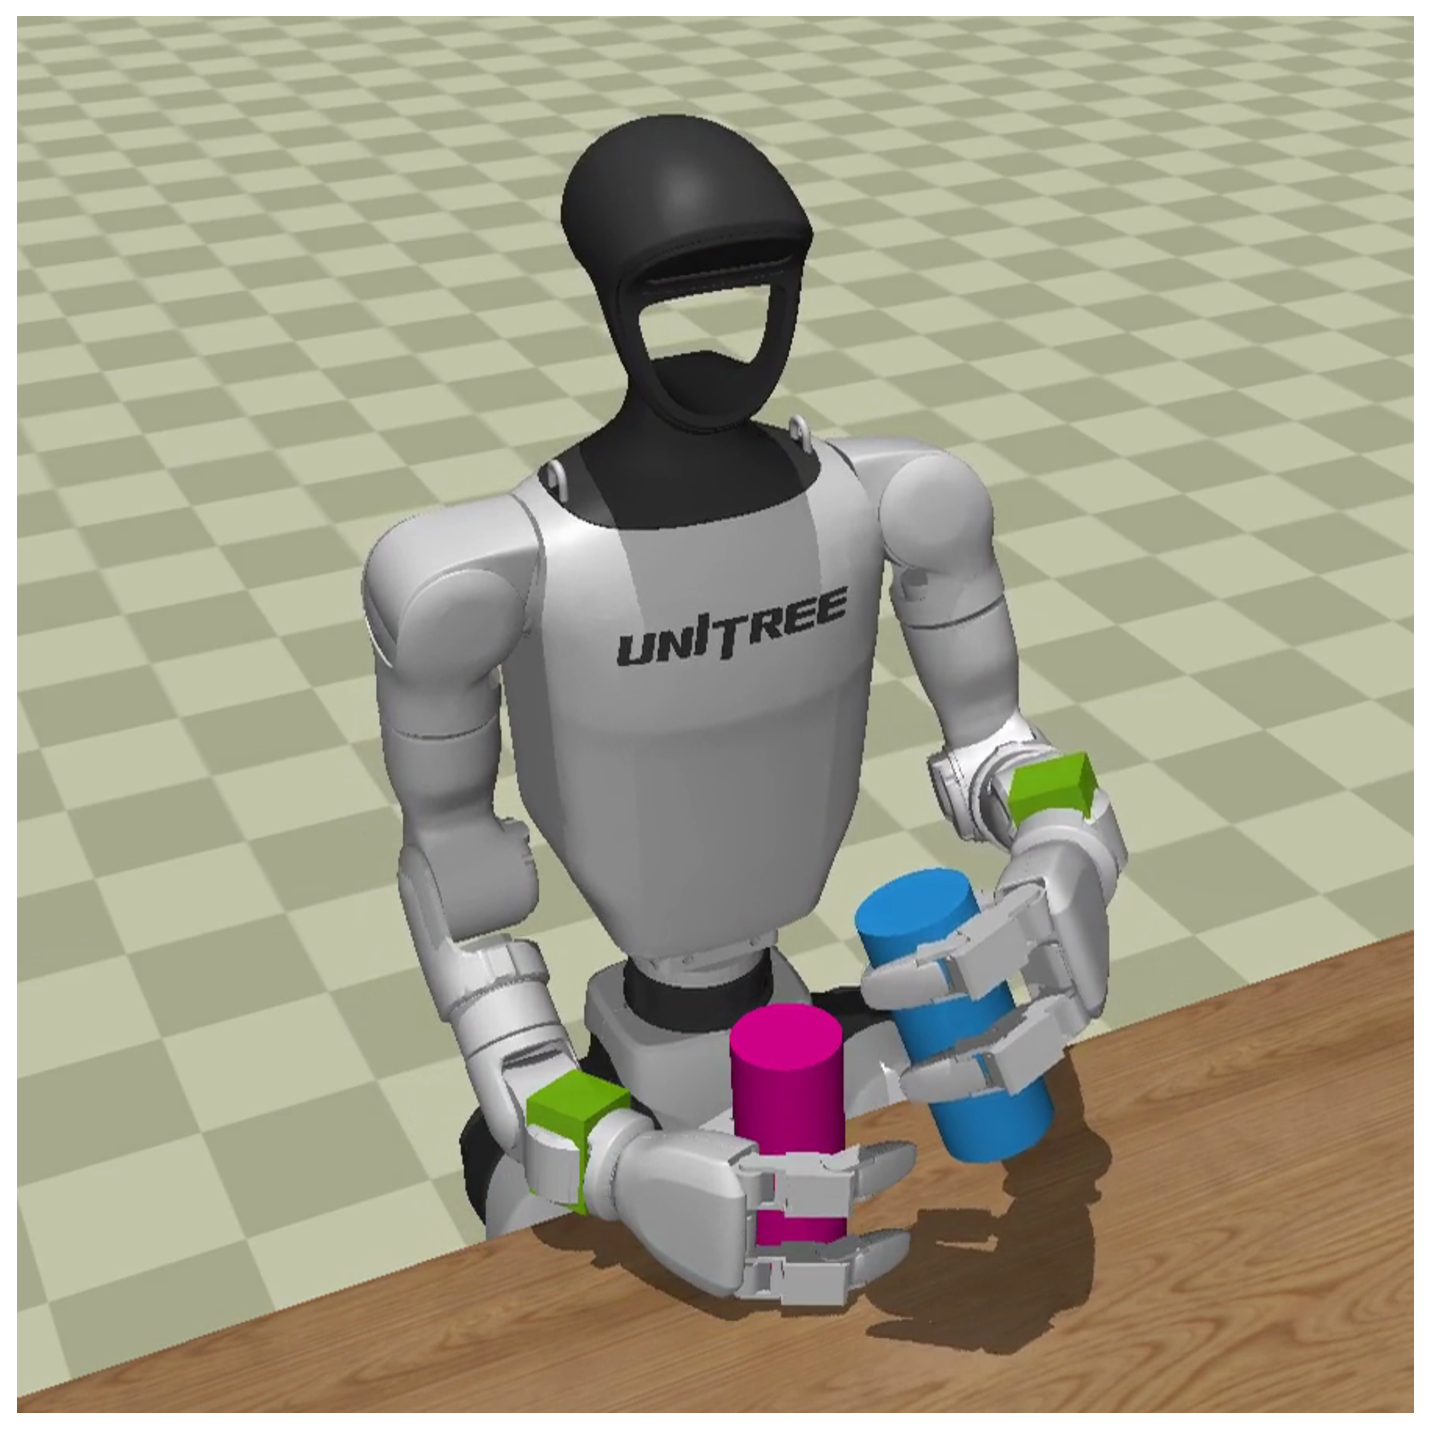
\includegraphics[width=0.16\textwidth]{figs/mujoco_g1.eps}
  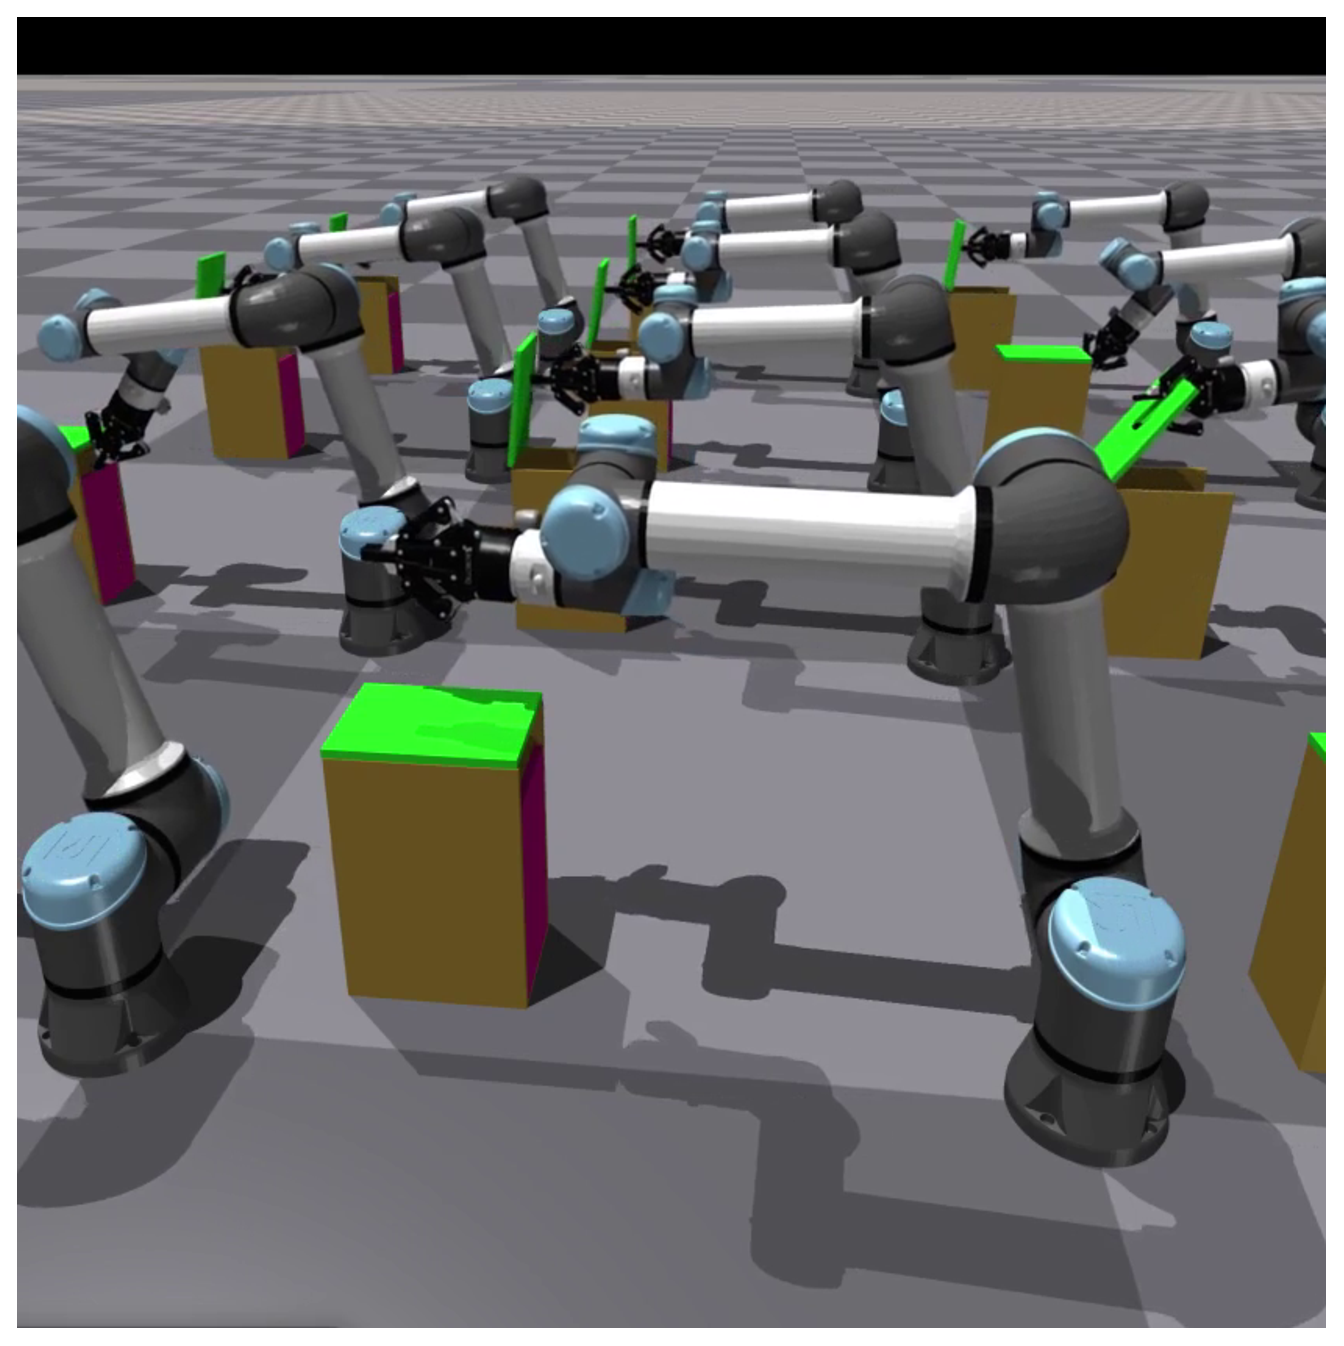
\includegraphics[width=0.16\textwidth]{figs/isaac_ur5e_parallel.eps}
  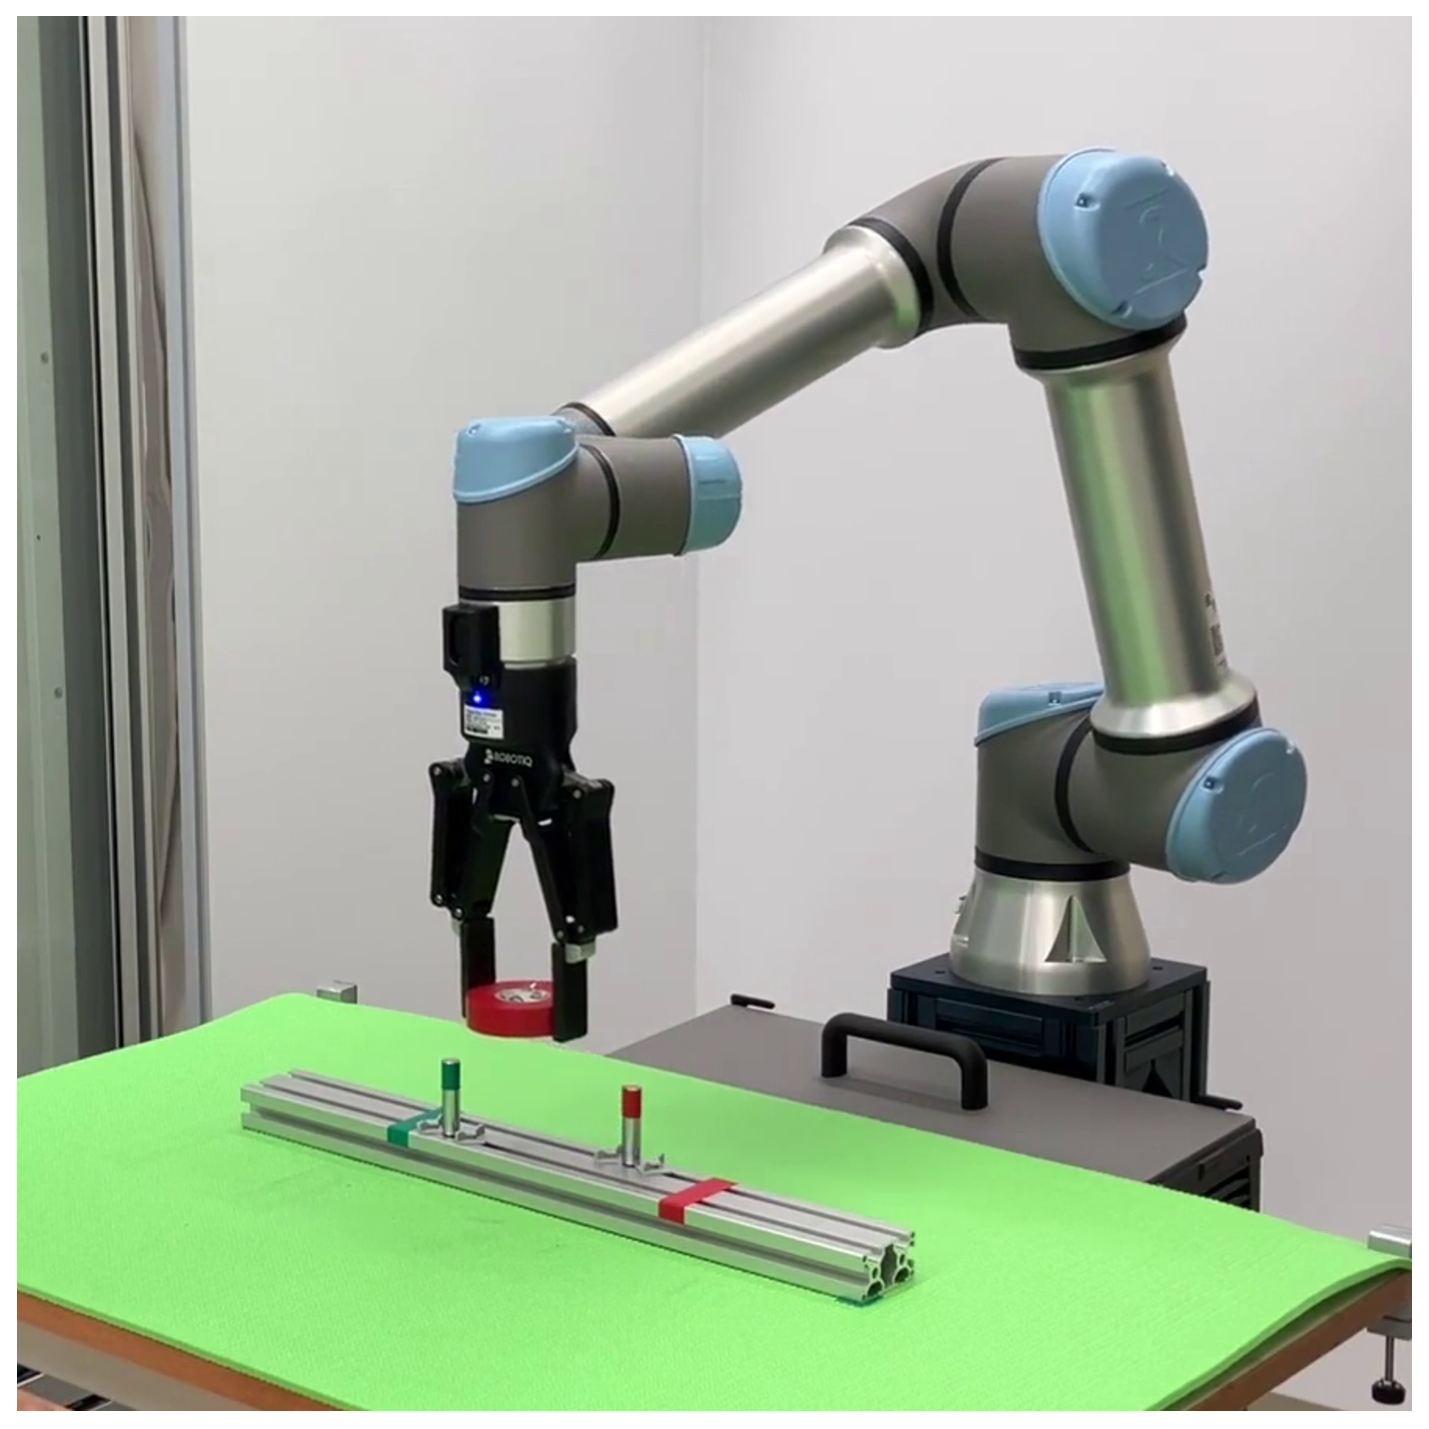
\includegraphics[width=0.16\textwidth]{figs/real_ur5e.eps}\\
  \begin{minipage}{0.16\textwidth}
    \begin{center} \footnotesize UR5e in MuJoCo \end{center}
  \end{minipage}
  \begin{minipage}{0.16\textwidth}
    \begin{center} \footnotesize ALOHA in MuJoCo \end{center}
  \end{minipage}
  \begin{minipage}{0.16\textwidth}
    \begin{center} \footnotesize HSR in MuJoCo \end{center}
  \end{minipage}
  \begin{minipage}{0.16\textwidth}
    \begin{center} \footnotesize G1 in MuJoCo \end{center}
  \end{minipage}
  \begin{minipage}[t]{0.16\textwidth}
    \begin{center} \footnotesize UR5e in Isaac Gym \end{center}
    %% \begin{center} \footnotesize UR5e in Isaac Gym\\ (parallel simulation) \end{center}
  \end{minipage}
  \begin{minipage}{0.16\textwidth}
    \begin{center} \footnotesize UR5e real robot \end{center}
  \end{minipage}
  \vspace{-1mm}
  \caption{Robot manipulation in simulation and real environments.}
  \label{fig:env}
  \vspace{-3mm}
\end{figure*}

The key components of robot imitation learning are the environment $\mathcal{E}$, dataset $\mathcal{D}$, and policy $\pi$.
For each, we describe how RoboManipBaselines ensures the principles of integration, generality, extensibility, and reproducibility.

\subsection{Environment}

RoboManipBaselines provides robot manipulation environments with an OpenAI Gym~\cite{OpenAIGym:Brockman:arXiv2016}-compatible interface for the real world, MuJoCo~\cite{MuJoCo:Todorov:IROS2012}, and Isaac Gym~\cite{IsaacGym:Makoviychuk:NeurIPS2021}.
As shown in \figref{fig:env}, it supports a wide range of robot embodiments, from single-arm manipulators (UR5e, xArm7) to bimanual (ALOHA, G1) and mobile manipulators (HSR).
By unifying real and simulated robots under the same interface, code validated in simulation can be directly applied to real hardware, and datasets from both domains can be seamlessly combined for training.
The simulation environments also support deformable objects such as ropes and cloth, offering more than ten dexterous manipulation tasks.
New simulators, robots, or tasks can be easily integrated by inheriting the abstract environment class and overriding a small number of methods.

\subsection{Dataset}

RoboManipBaselines publishes pre-collected datasets to support reproducible benchmarking.
In simulation, models can be trained and evaluated directly with these datasets, facilitating systematic comparison of new methods.
It also supports additional data collection through various teleoperation interfaces such as keyboard, 3D mouse, and leader-follower system GELLO~\cite{GELLO:Wu:IROS2024}.
The environment abstraction enables teleoperation to be carried out in an identical way across real and simulated robots.
The custom data format balances compression and I/O, and accommodates multimodal signals including joint states, RGB-D images, and force/torque or tactile measurements.
Moreover, absolute and relative representations of joint and end-effector states are stored independently, enabling flexible definition of state and action spaces for policy training.

\subsection{Policy}

RoboManipBaselines unifies training and rollout of a wide range of policy model architectures, including ACT~\cite{ALOHA:Zhao:RSS2023}, Diffusion Policy~\cite{DiffusionPolicy:Chi:IJRR2024}, and SARNN~\cite{SARNN:Ichiwara:ICRA2022}.
It also supports 3D Diffusion Policy~\cite{3DDiffusionPolicy:Ze:RSS2024}, which takes 3D point clouds as input, and MT-ACT~\cite{MtAct:Bharadhwaj:ICRA2024}, which flexibly executes multiple tasks from language instructions, demonstrating generality with respect to multimodal sensing and diverse tasks.
%% Thanks to the environment abstraction, policy deployment is unified across real and simulated robots.
%% New policies can be easily added by inheriting the abstract classes for training and rollout and overriding only a few methods, ensuring high extensibility.


%%%%%%%%%%%%%%%%%%%%%%%%%%%%%%%%%%%%%%%%%%%%%%%%%%%%%%%%%%%%%%%%%%%%%%%%%%%%%%%%
\section{Evaluation}

\begin{table}[t]
  \centering
  \caption{Task success rates (mean $\pm$ std).}
  \label{tab:eval}
  \vspace{-2mm}
  \begin{tabular}{lcc}
    \toprule
    Policy & Real-world & Simulation \\
    \midrule
    ACT~\cite{ALOHA:Zhao:RSS2023} & 0.54 $\pm$ 0.51 & 0.79 $\pm$ 0.41 \\
    Diffusion Policy~\cite{DiffusionPolicy:Chi:IJRR2024} & 0.58 $\pm$ 0.50 & 0.71 $\pm$ 0.46 \\
    SARNN~\cite{SARNN:Ichiwara:ICRA2022} & 0.63 $\pm$ 0.50 & 1.00 $\pm$ 0.0 \\
    \bottomrule
  \end{tabular}
\end{table}

Using RoboManipBaselines, we evaluated multiple policies on UR5e manipulation tasks in real and MuJoCo environments.
Each environment included four tasks with challenging objects.
\tabref{tab:eval} shows success rates of three policies.
Policies were trained from 30 teleoperation data with initial object positions randomized within 10 cm, and evaluated with six rollouts in the real world and 60 in simulation.
The results confirm the effectiveness of RoboManipBaselines for difficult tasks and underscore the value of a general framework for systematic comparison of diverse methods.


%%%%%%%%%%%%%%%%%%%%%%%%%%%%%%%%%%%%%%%%%%%%%%%%%%%%%%%%%%%%%%%%%%%%%%%%%%%%%%%%
\section{Conclusion}

We introduced RoboManipBaselines, a unified framework for robotic imitation learning in simulation and real environments. Emphasizing integration, generality, extensibility, and reproducibility, it enables end-to-end workflows and systematic benchmarking of robots, tasks, and policies. We will further extend it toward large-scale robotic foundation models~\cite{pi0:Black:arXiv2024,GR00T:Bjorck:arXiv2025} and broader applications.


%%%%%%%%%%%%%%%%%%%%%%%%%%%%%%%%%%%%%%%%%%%%%%%%%%%%%%%%%%%%%%%%%%%%%%%%%%%%%%%%
\clearpage
\onecolumn
\twocolumn
\balance
\bibliographystyle{IEEEtran}
\bibliography{main.bib}

\end{document}
